% Software Development for Mobile Devices
\documentclass[11pt,english,numbers=endperiod,parskip=full]{scrartcl}

\usepackage{color}
\usepackage{graphicx}
\usepackage{minted}

\definecolor{gray}{rgb}{0.4,0.4,0.4}
\definecolor{darkblue}{rgb}{0.0,0.0,0.6}
\definecolor{cyan}{rgb}{0.0,0.6,0.6}

\title{Assignment 01}
\subtitle{COS30017 - Software Development for Mobile Devices}
\author{Daniel Parker 971328X}

\date{\today}

\begin{document}
\maketitle

\section{Task 1}
\subsection{Source}
\subsubsection{activity\_melbourne.xml}
\inputminted{xml}{../../Apps/Melbourne/app/src/main/res/layout/activity_melbourne.xml}

\subsubsection{strings.xml}
\inputminted{xml}{../../Apps/Melbourne/app/src/main/res/values/strings.xml}

\subsection{Screenshots}
\setlength\fboxsep{0pt}
\setlength\fboxrule{0.5pt}
\centering{
	\fbox{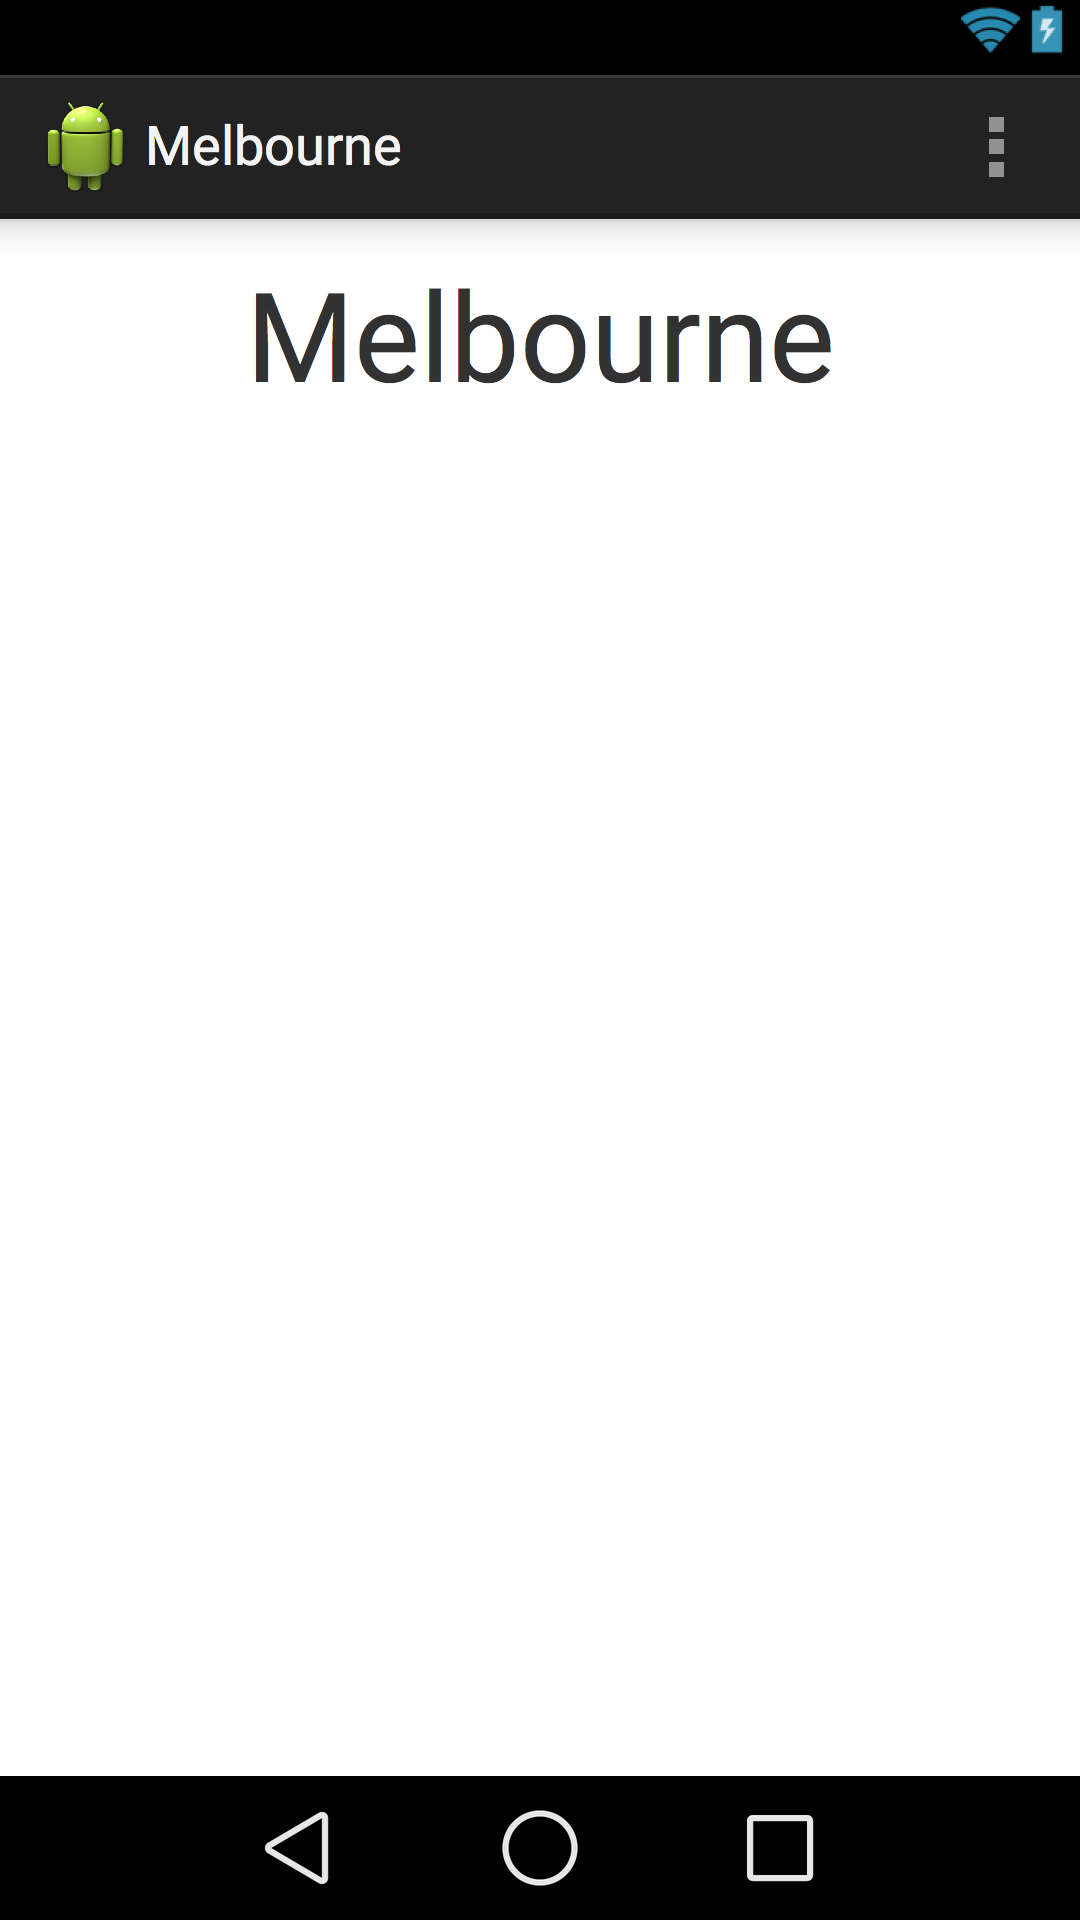
\includegraphics[width=5cm]{../../Apps/Melbourne/Assignment/Melbourne-portrait.png}}
}\\
\bigskip
\centering{
	\fbox{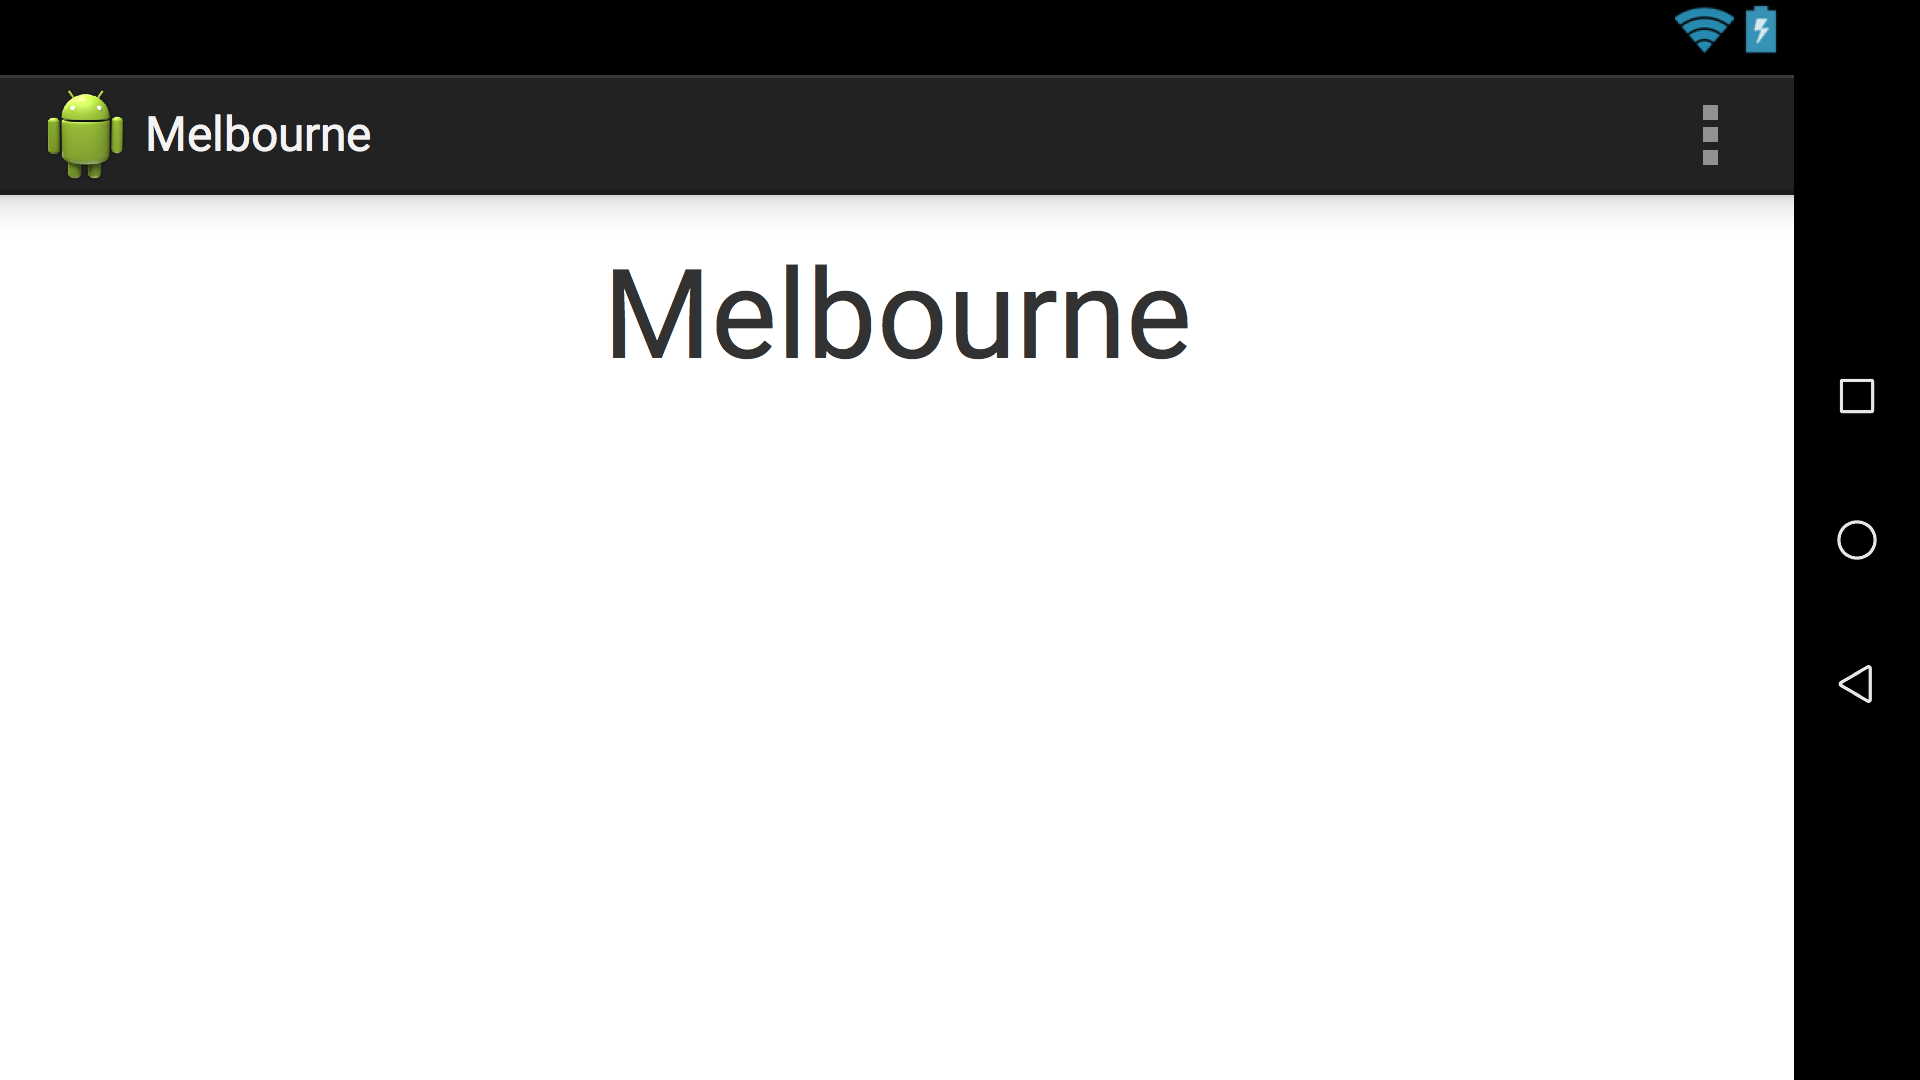
\includegraphics[width=10cm]{../../Apps/Melbourne/Assignment/Melbourne-landscape.png}}
}
\\

\section{Task 2}
\raggedright
A common design paradigm used in the software industry is that of convention over configuration. The purpose of convention over configuration is to reduce the number of decisions that have to be made by developers by providing a series of conventions as solutions for recurring decisions. Some examples are naming conventions, project structure conventions and coding conventions.

Android development encourages use of conventions, so much so that Android Studio, the integrated development environment developed by Google for Android development, will ensure certain conventions are followed and generate code automatically that follows those conventions.

The Android developer documentation recommends a naming convention for icon files as shown in this screenshot from the website.

\centering{
	\fbox{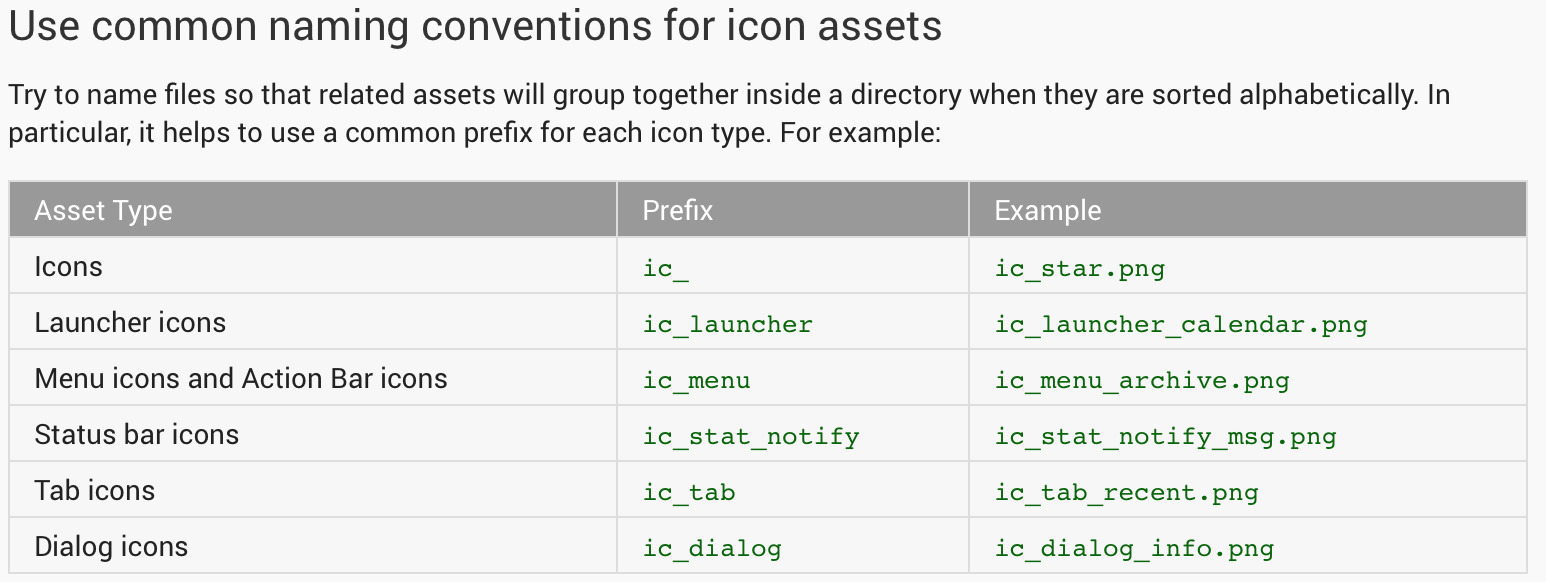
\includegraphics[width=15cm]{images/icon-naming.png}
}\\

\raggedright
Another good example of convention used in Android development is the structure of the project as generated by Android Studio when a project is setup. In the screenshot below we can see that the 'src' directory contains all the program source code but divided into java code in the 'java' directory and resources (such as images and XML) in the 'res' directory. Further directory conventions are used within each directory, all the way down to different drawable directories for different screen pixel densities.

\centering{
	\fbox{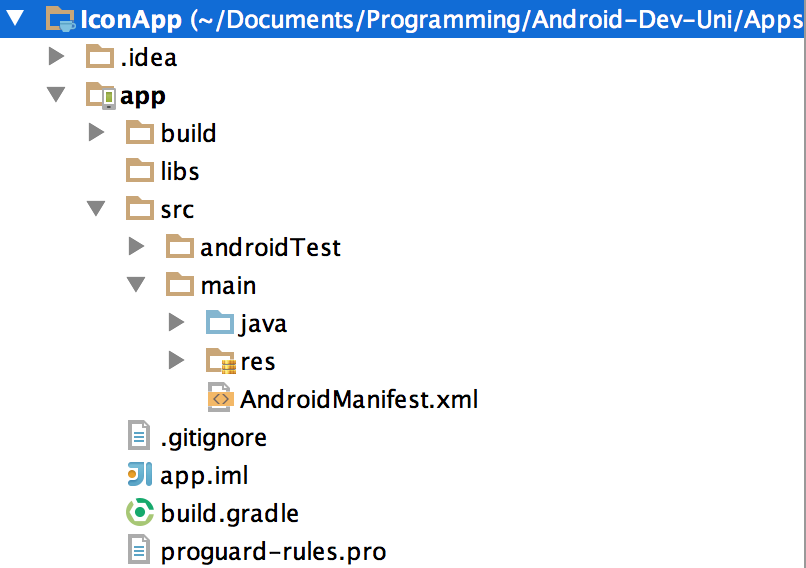
\includegraphics[width=10cm]{images/Project-Structure.png}
}\\

\section{Task 3}
\subsection{Source}
\subsubsection{activity\_icon.xml}
\inputminted{xml}{../../Apps/IconApp/app/src/main/res/layout/activity_icon.xml}

\subsection{Screenshots}
\subsubsection{mdpi}
\centering{
	\fbox{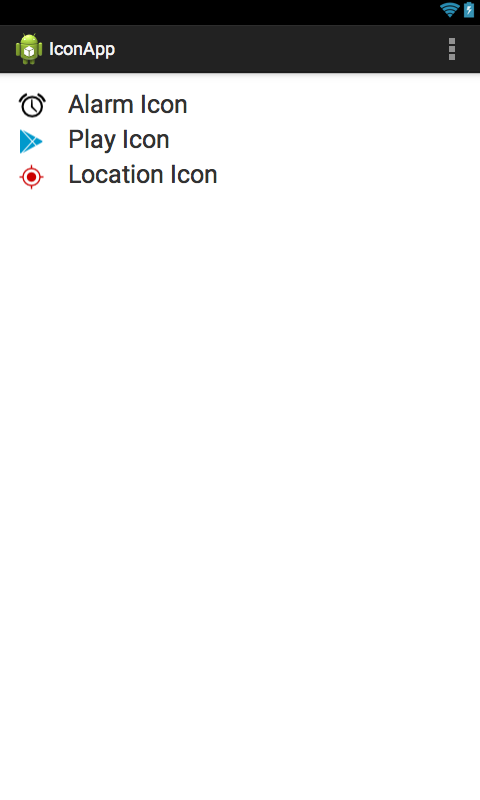
\includegraphics[width=5cm]{../../Apps/IconApp/Assignment/mdpi.png}}
}\\
\bigskip

\subsubsection{hdpi}
\centering{
	\fbox{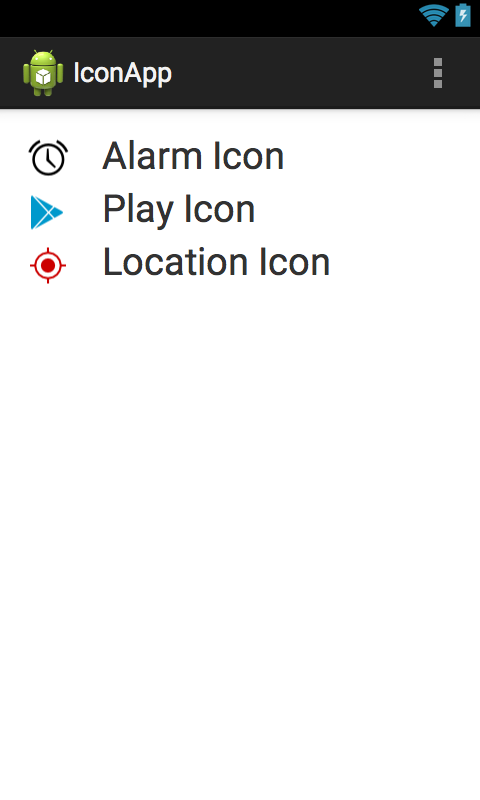
\includegraphics[width=5cm]{../../Apps/IconApp/Assignment/hdpi.png}}
}\\
\bigskip

\subsubsection{xxhdpi}
\centering{
	\fbox{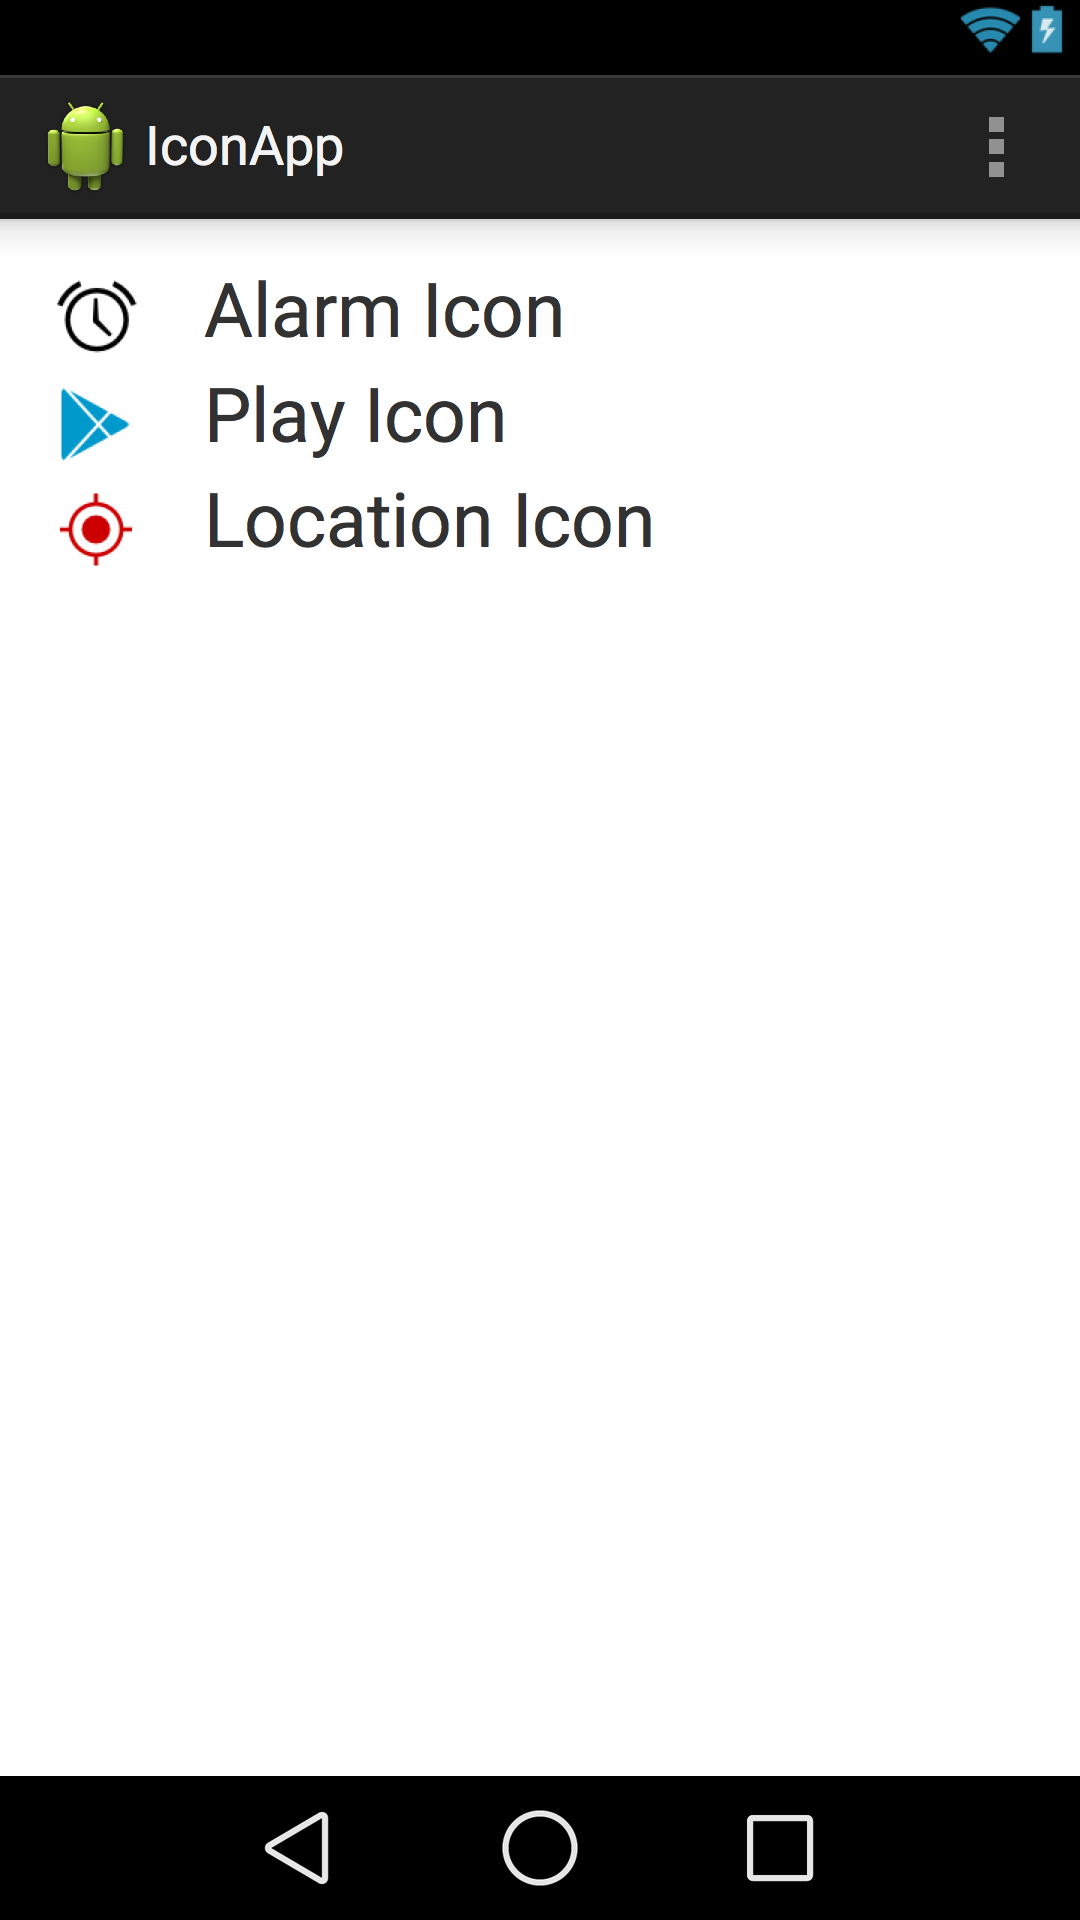
\includegraphics[width=5cm]{../../Apps/IconApp/Assignment/xxhdpi.png}}
}\\
\bigskip

\subsection{Low density icon on XXHDPI screen}
\raggedright
It is possible to force a high density screen to show a low density icon but the icon will either display much smaller than it should be or it will be the correct size but look pixelated. That will be determined by whether the XML defines sized in 'dp' or 'px'. 'dp' sizes will scale proportionally based on the device's pixel density. The screenshot below shows how the low density alarm image will look smaller on a high density screen. 

\centering{
	\fbox{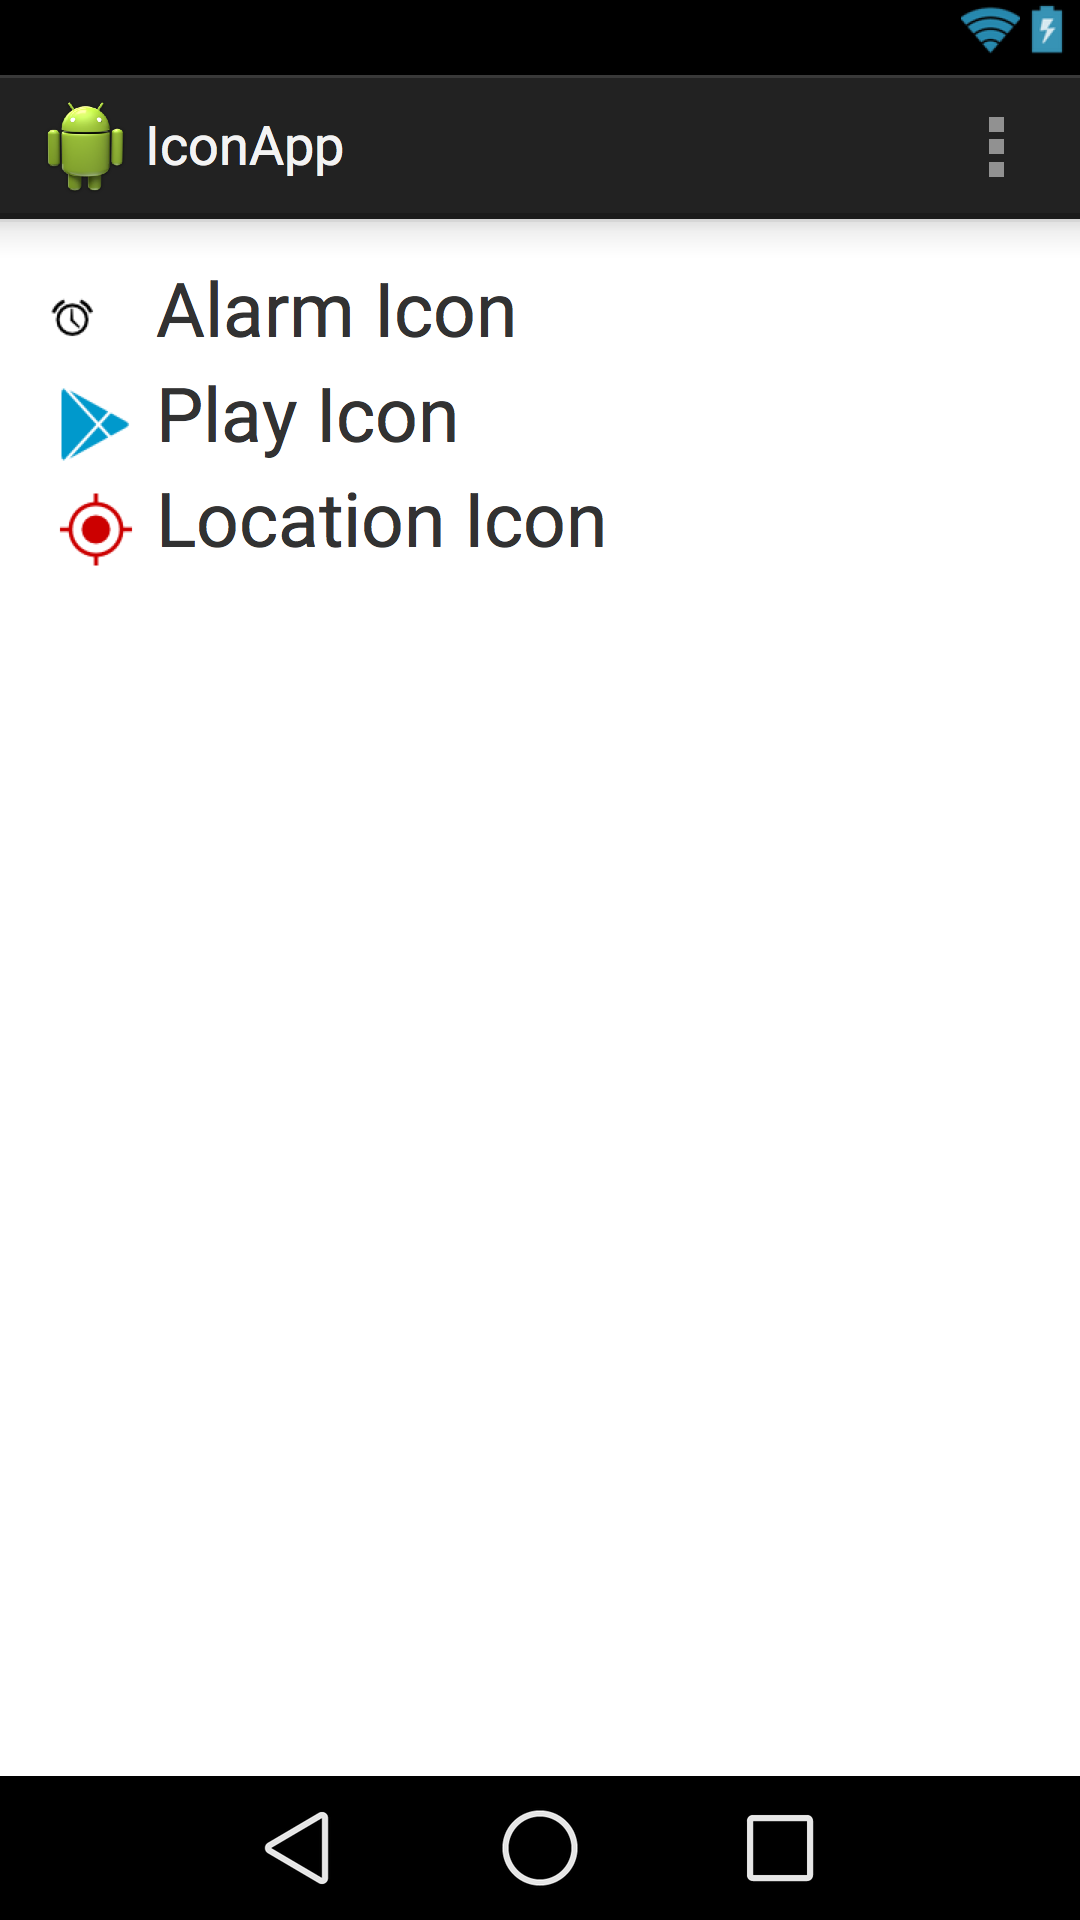
\includegraphics[width=5cm]{../../Apps/IconApp/Assignment/incorrect-size.png}}
}\\
\bigskip

\section{Task 4}
\raggedright{There is a need to use device independent font sizing because:}\\
\begin{itemize}
	\item The pixel density is different between devices.
	\item Fonts will not show correctly across different devices if device dependent font sizing is used, ie. 'px' instead of 'sp'.
	\item Fonts need to scale correctly so that they are readable on different density screens.

\end{itemize}

\end{document}
